% Options for packages loaded elsewhere
\PassOptionsToPackage{unicode}{hyperref}
\PassOptionsToPackage{hyphens}{url}
%
\documentclass[
]{article}
\usepackage{amsmath,amssymb}
\usepackage{lmodern}
\usepackage{iftex}
\ifPDFTeX
  \usepackage[T1]{fontenc}
  \usepackage[utf8]{inputenc}
  \usepackage{textcomp} % provide euro and other symbols
\else % if luatex or xetex
  \usepackage{unicode-math}
  \defaultfontfeatures{Scale=MatchLowercase}
  \defaultfontfeatures[\rmfamily]{Ligatures=TeX,Scale=1}
\fi
% Use upquote if available, for straight quotes in verbatim environments
\IfFileExists{upquote.sty}{\usepackage{upquote}}{}
\IfFileExists{microtype.sty}{% use microtype if available
  \usepackage[]{microtype}
  \UseMicrotypeSet[protrusion]{basicmath} % disable protrusion for tt fonts
}{}
\makeatletter
\@ifundefined{KOMAClassName}{% if non-KOMA class
  \IfFileExists{parskip.sty}{%
    \usepackage{parskip}
  }{% else
    \setlength{\parindent}{0pt}
    \setlength{\parskip}{6pt plus 2pt minus 1pt}}
}{% if KOMA class
  \KOMAoptions{parskip=half}}
\makeatother
\usepackage{xcolor}
\usepackage[margin=1in]{geometry}
\usepackage{color}
\usepackage{fancyvrb}
\newcommand{\VerbBar}{|}
\newcommand{\VERB}{\Verb[commandchars=\\\{\}]}
\DefineVerbatimEnvironment{Highlighting}{Verbatim}{commandchars=\\\{\}}
% Add ',fontsize=\small' for more characters per line
\usepackage{framed}
\definecolor{shadecolor}{RGB}{248,248,248}
\newenvironment{Shaded}{\begin{snugshade}}{\end{snugshade}}
\newcommand{\AlertTok}[1]{\textcolor[rgb]{0.94,0.16,0.16}{#1}}
\newcommand{\AnnotationTok}[1]{\textcolor[rgb]{0.56,0.35,0.01}{\textbf{\textit{#1}}}}
\newcommand{\AttributeTok}[1]{\textcolor[rgb]{0.77,0.63,0.00}{#1}}
\newcommand{\BaseNTok}[1]{\textcolor[rgb]{0.00,0.00,0.81}{#1}}
\newcommand{\BuiltInTok}[1]{#1}
\newcommand{\CharTok}[1]{\textcolor[rgb]{0.31,0.60,0.02}{#1}}
\newcommand{\CommentTok}[1]{\textcolor[rgb]{0.56,0.35,0.01}{\textit{#1}}}
\newcommand{\CommentVarTok}[1]{\textcolor[rgb]{0.56,0.35,0.01}{\textbf{\textit{#1}}}}
\newcommand{\ConstantTok}[1]{\textcolor[rgb]{0.00,0.00,0.00}{#1}}
\newcommand{\ControlFlowTok}[1]{\textcolor[rgb]{0.13,0.29,0.53}{\textbf{#1}}}
\newcommand{\DataTypeTok}[1]{\textcolor[rgb]{0.13,0.29,0.53}{#1}}
\newcommand{\DecValTok}[1]{\textcolor[rgb]{0.00,0.00,0.81}{#1}}
\newcommand{\DocumentationTok}[1]{\textcolor[rgb]{0.56,0.35,0.01}{\textbf{\textit{#1}}}}
\newcommand{\ErrorTok}[1]{\textcolor[rgb]{0.64,0.00,0.00}{\textbf{#1}}}
\newcommand{\ExtensionTok}[1]{#1}
\newcommand{\FloatTok}[1]{\textcolor[rgb]{0.00,0.00,0.81}{#1}}
\newcommand{\FunctionTok}[1]{\textcolor[rgb]{0.00,0.00,0.00}{#1}}
\newcommand{\ImportTok}[1]{#1}
\newcommand{\InformationTok}[1]{\textcolor[rgb]{0.56,0.35,0.01}{\textbf{\textit{#1}}}}
\newcommand{\KeywordTok}[1]{\textcolor[rgb]{0.13,0.29,0.53}{\textbf{#1}}}
\newcommand{\NormalTok}[1]{#1}
\newcommand{\OperatorTok}[1]{\textcolor[rgb]{0.81,0.36,0.00}{\textbf{#1}}}
\newcommand{\OtherTok}[1]{\textcolor[rgb]{0.56,0.35,0.01}{#1}}
\newcommand{\PreprocessorTok}[1]{\textcolor[rgb]{0.56,0.35,0.01}{\textit{#1}}}
\newcommand{\RegionMarkerTok}[1]{#1}
\newcommand{\SpecialCharTok}[1]{\textcolor[rgb]{0.00,0.00,0.00}{#1}}
\newcommand{\SpecialStringTok}[1]{\textcolor[rgb]{0.31,0.60,0.02}{#1}}
\newcommand{\StringTok}[1]{\textcolor[rgb]{0.31,0.60,0.02}{#1}}
\newcommand{\VariableTok}[1]{\textcolor[rgb]{0.00,0.00,0.00}{#1}}
\newcommand{\VerbatimStringTok}[1]{\textcolor[rgb]{0.31,0.60,0.02}{#1}}
\newcommand{\WarningTok}[1]{\textcolor[rgb]{0.56,0.35,0.01}{\textbf{\textit{#1}}}}
\usepackage{graphicx}
\makeatletter
\def\maxwidth{\ifdim\Gin@nat@width>\linewidth\linewidth\else\Gin@nat@width\fi}
\def\maxheight{\ifdim\Gin@nat@height>\textheight\textheight\else\Gin@nat@height\fi}
\makeatother
% Scale images if necessary, so that they will not overflow the page
% margins by default, and it is still possible to overwrite the defaults
% using explicit options in \includegraphics[width, height, ...]{}
\setkeys{Gin}{width=\maxwidth,height=\maxheight,keepaspectratio}
% Set default figure placement to htbp
\makeatletter
\def\fps@figure{htbp}
\makeatother
\setlength{\emergencystretch}{3em} % prevent overfull lines
\providecommand{\tightlist}{%
  \setlength{\itemsep}{0pt}\setlength{\parskip}{0pt}}
\setcounter{secnumdepth}{-\maxdimen} % remove section numbering
\usepackage{booktabs}
\usepackage{longtable}
\usepackage{array}
\usepackage{multirow}
\usepackage{wrapfig}
\usepackage{float}
\usepackage{colortbl}
\usepackage{pdflscape}
\usepackage{tabu}
\usepackage{threeparttable}
\usepackage{threeparttablex}
\usepackage[normalem]{ulem}
\usepackage{makecell}
\usepackage{xcolor}
\ifLuaTeX
  \usepackage{selnolig}  % disable illegal ligatures
\fi
\IfFileExists{bookmark.sty}{\usepackage{bookmark}}{\usepackage{hyperref}}
\IfFileExists{xurl.sty}{\usepackage{xurl}}{} % add URL line breaks if available
\urlstyle{same} % disable monospaced font for URLs
\hypersetup{
  pdftitle={Midterm},
  pdfauthor={Mahathi Gandhamaneni},
  hidelinks,
  pdfcreator={LaTeX via pandoc}}

\title{Midterm}
\author{Mahathi Gandhamaneni}
\date{}

\begin{document}
\maketitle

\begin{Shaded}
\begin{Highlighting}[]
\FunctionTok{library}\NormalTok{(httr)}
\FunctionTok{library}\NormalTok{(tidyverse)}
\end{Highlighting}
\end{Shaded}

\begin{verbatim}
## -- Attaching packages --------------------------------------- tidyverse 1.3.2 --
## v ggplot2 3.4.0      v purrr   1.0.0 
## v tibble  3.1.8      v dplyr   1.0.10
## v tidyr   1.2.1      v stringr 1.5.0 
## v readr   2.1.3      v forcats 0.5.2 
## -- Conflicts ------------------------------------------ tidyverse_conflicts() --
## x dplyr::filter() masks stats::filter()
## x dplyr::lag()    masks stats::lag()
\end{verbatim}

\begin{Shaded}
\begin{Highlighting}[]
\FunctionTok{library}\NormalTok{(xml2)}
\FunctionTok{library}\NormalTok{(stringr)}
\FunctionTok{library}\NormalTok{(knitr)}
\FunctionTok{library}\NormalTok{(vtable)}
\end{Highlighting}
\end{Shaded}

\begin{verbatim}
## Loading required package: kableExtra
\end{verbatim}

\begin{verbatim}
## Warning in !is.null(rmarkdown::metadata$output) && rmarkdown::metadata$output
## %in% : 'length(x) = 3 > 1' in coercion to 'logical(1)'
\end{verbatim}

\begin{verbatim}
## 
## Attaching package: 'kableExtra'
## 
## The following object is masked from 'package:dplyr':
## 
##     group_rows
\end{verbatim}

\begin{Shaded}
\begin{Highlighting}[]
\NormalTok{life\_expectancy }\OtherTok{\textless{}{-}} \FunctionTok{data.frame}\NormalTok{()}

\CommentTok{\# List of countries to scrape}
\NormalTok{countries }\OtherTok{\textless{}{-}} \FunctionTok{c}\NormalTok{(}\StringTok{"PRT"}\NormalTok{, }\StringTok{"DEU"}\NormalTok{, }\StringTok{"ESP"}\NormalTok{, }\StringTok{"ITA"}\NormalTok{, }\StringTok{"NLD"}\NormalTok{, }\StringTok{"GBR"}\NormalTok{, }\StringTok{"LTU"}\NormalTok{, }\StringTok{"AGO"}\NormalTok{, }\StringTok{"CPV"}\NormalTok{, }\StringTok{"GIN"}\NormalTok{, }\StringTok{"MOZ"}\NormalTok{, }\StringTok{"STP"}\NormalTok{, }\StringTok{"TUR"}\NormalTok{, }\StringTok{"BRA"}\NormalTok{, }\StringTok{"ROU"}\NormalTok{, }\StringTok{"MDA"}\NormalTok{, }\StringTok{"MEX"}\NormalTok{, }\StringTok{"UKR"}\NormalTok{, }\StringTok{"RUS"}\NormalTok{, }\StringTok{"CUB"}\NormalTok{, }\StringTok{"COL"}\NormalTok{)}

\ControlFlowTok{for}\NormalTok{ (i }\ControlFlowTok{in} \DecValTok{1}\SpecialCharTok{:}\FunctionTok{length}\NormalTok{(countries)) \{}
\NormalTok{  url }\OtherTok{\textless{}{-}} \FunctionTok{paste0}\NormalTok{(}\StringTok{"http://api.worldbank.org/v2/country/"}\NormalTok{, }\FunctionTok{tolower}\NormalTok{(}\FunctionTok{gsub}\NormalTok{(}\StringTok{" "}\NormalTok{, }\StringTok{"\%20"}\NormalTok{, countries[i])), }\StringTok{"/indicator/SP.DYN.LE00.IN?date=2019"}\NormalTok{)}

\NormalTok{restaurant\_license\_xml }\OtherTok{=} \FunctionTok{as\_list}\NormalTok{(}\FunctionTok{read\_xml}\NormalTok{(url))}

\NormalTok{xml\_df }\OtherTok{=}\NormalTok{ tibble}\SpecialCharTok{::}\FunctionTok{as\_tibble}\NormalTok{(restaurant\_license\_xml) }\SpecialCharTok{\%\textgreater{}\%}
  \FunctionTok{unnest\_wider}\NormalTok{(data)}

\NormalTok{lp\_df }\OtherTok{=}\NormalTok{ xml\_df }\SpecialCharTok{\%\textgreater{}\%}
  \FunctionTok{unnest}\NormalTok{(}\AttributeTok{cols =} \FunctionTok{names}\NormalTok{(.)) }\SpecialCharTok{\%\textgreater{}\%}
  \FunctionTok{unnest}\NormalTok{(}\AttributeTok{cols =} \FunctionTok{names}\NormalTok{(.)) }\SpecialCharTok{\%\textgreater{}\%}
  \CommentTok{\# convert data type}
\NormalTok{  readr}\SpecialCharTok{::}\FunctionTok{type\_convert}\NormalTok{()}

\CommentTok{\# lp\_df \textless{}{-} lp\_df \%\textgreater{}\% unnest\_wider(data\_id)}

\NormalTok{life\_expectancy }\OtherTok{\textless{}{-}} \FunctionTok{bind\_rows}\NormalTok{(life\_expectancy, lp\_df)}

\NormalTok{\}}
\end{Highlighting}
\end{Shaded}

\begin{verbatim}
## 
## -- Column specification --------------------------------------------------------
## cols(
##   indicator = col_character(),
##   country = col_character(),
##   countryiso3code = col_character(),
##   date = col_double(),
##   value = col_double(),
##   decimal = col_double()
## )
## 
## 
## -- Column specification --------------------------------------------------------
## cols(
##   indicator = col_character(),
##   country = col_character(),
##   countryiso3code = col_character(),
##   date = col_double(),
##   value = col_double(),
##   decimal = col_double()
## )
## 
## 
## -- Column specification --------------------------------------------------------
## cols(
##   indicator = col_character(),
##   country = col_character(),
##   countryiso3code = col_character(),
##   date = col_double(),
##   value = col_double(),
##   decimal = col_double()
## )
## 
## 
## -- Column specification --------------------------------------------------------
## cols(
##   indicator = col_character(),
##   country = col_character(),
##   countryiso3code = col_character(),
##   date = col_double(),
##   value = col_double(),
##   decimal = col_double()
## )
## 
## 
## -- Column specification --------------------------------------------------------
## cols(
##   indicator = col_character(),
##   country = col_character(),
##   countryiso3code = col_character(),
##   date = col_double(),
##   value = col_double(),
##   decimal = col_double()
## )
## 
## 
## -- Column specification --------------------------------------------------------
## cols(
##   indicator = col_character(),
##   country = col_character(),
##   countryiso3code = col_character(),
##   date = col_double(),
##   value = col_double(),
##   decimal = col_double()
## )
## 
## 
## -- Column specification --------------------------------------------------------
## cols(
##   indicator = col_character(),
##   country = col_character(),
##   countryiso3code = col_character(),
##   date = col_double(),
##   value = col_double(),
##   decimal = col_double()
## )
## 
## 
## -- Column specification --------------------------------------------------------
## cols(
##   indicator = col_character(),
##   country = col_character(),
##   countryiso3code = col_character(),
##   date = col_double(),
##   value = col_double(),
##   decimal = col_double()
## )
## 
## 
## -- Column specification --------------------------------------------------------
## cols(
##   indicator = col_character(),
##   country = col_character(),
##   countryiso3code = col_character(),
##   date = col_double(),
##   value = col_double(),
##   decimal = col_double()
## )
## 
## 
## -- Column specification --------------------------------------------------------
## cols(
##   indicator = col_character(),
##   country = col_character(),
##   countryiso3code = col_character(),
##   date = col_double(),
##   value = col_double(),
##   decimal = col_double()
## )
## 
## 
## -- Column specification --------------------------------------------------------
## cols(
##   indicator = col_character(),
##   country = col_character(),
##   countryiso3code = col_character(),
##   date = col_double(),
##   value = col_double(),
##   decimal = col_double()
## )
## 
## 
## -- Column specification --------------------------------------------------------
## cols(
##   indicator = col_character(),
##   country = col_character(),
##   countryiso3code = col_character(),
##   date = col_double(),
##   value = col_double(),
##   decimal = col_double()
## )
## 
## 
## -- Column specification --------------------------------------------------------
## cols(
##   indicator = col_character(),
##   country = col_character(),
##   countryiso3code = col_character(),
##   date = col_double(),
##   value = col_double(),
##   decimal = col_double()
## )
## 
## 
## -- Column specification --------------------------------------------------------
## cols(
##   indicator = col_character(),
##   country = col_character(),
##   countryiso3code = col_character(),
##   date = col_double(),
##   value = col_double(),
##   decimal = col_double()
## )
## 
## 
## -- Column specification --------------------------------------------------------
## cols(
##   indicator = col_character(),
##   country = col_character(),
##   countryiso3code = col_character(),
##   date = col_double(),
##   value = col_double(),
##   decimal = col_double()
## )
## 
## 
## -- Column specification --------------------------------------------------------
## cols(
##   indicator = col_character(),
##   country = col_character(),
##   countryiso3code = col_character(),
##   date = col_double(),
##   value = col_double(),
##   decimal = col_double()
## )
## 
## 
## -- Column specification --------------------------------------------------------
## cols(
##   indicator = col_character(),
##   country = col_character(),
##   countryiso3code = col_character(),
##   date = col_double(),
##   value = col_double(),
##   decimal = col_double()
## )
## 
## 
## -- Column specification --------------------------------------------------------
## cols(
##   indicator = col_character(),
##   country = col_character(),
##   countryiso3code = col_character(),
##   date = col_double(),
##   value = col_double(),
##   decimal = col_double()
## )
## 
## 
## -- Column specification --------------------------------------------------------
## cols(
##   indicator = col_character(),
##   country = col_character(),
##   countryiso3code = col_character(),
##   date = col_double(),
##   value = col_double(),
##   decimal = col_double()
## )
## 
## 
## -- Column specification --------------------------------------------------------
## cols(
##   indicator = col_character(),
##   country = col_character(),
##   countryiso3code = col_character(),
##   date = col_double(),
##   value = col_double(),
##   decimal = col_double()
## )
## 
## 
## -- Column specification --------------------------------------------------------
## cols(
##   indicator = col_character(),
##   country = col_character(),
##   countryiso3code = col_character(),
##   date = col_double(),
##   value = col_double(),
##   decimal = col_double()
## )
\end{verbatim}

\begin{Shaded}
\begin{Highlighting}[]
\NormalTok{life\_expectancy }\OtherTok{\textless{}{-}}\NormalTok{ life\_expectancy }\SpecialCharTok{\%\textgreater{}\%} \FunctionTok{select}\NormalTok{(countryiso3code, value)}
\NormalTok{life\_expectancy }\OtherTok{\textless{}{-}} \FunctionTok{cbind}\NormalTok{(}\AttributeTok{Nacionality =} \DecValTok{1}\SpecialCharTok{:}\FunctionTok{nrow}\NormalTok{(life\_expectancy), life\_expectancy)}

\NormalTok{df }\OtherTok{\textless{}{-}} \FunctionTok{read.csv}\NormalTok{(}\StringTok{"dataset.csv"}\NormalTok{)}

\CommentTok{\# Left join}
\NormalTok{df }\OtherTok{\textless{}{-}} \FunctionTok{merge}\NormalTok{(}\AttributeTok{x=}\NormalTok{df,}\AttributeTok{y=}\NormalTok{life\_expectancy, }
             \AttributeTok{by=}\StringTok{"Nacionality"}\NormalTok{, }\AttributeTok{all.x=}\ConstantTok{TRUE}\NormalTok{)}
\end{Highlighting}
\end{Shaded}

\begin{Shaded}
\begin{Highlighting}[]
\FunctionTok{dim}\NormalTok{(df)}
\end{Highlighting}
\end{Shaded}

\begin{verbatim}
## [1] 4424   37
\end{verbatim}

\begin{Shaded}
\begin{Highlighting}[]
\FunctionTok{head}\NormalTok{(df)}
\end{Highlighting}
\end{Shaded}

\begin{verbatim}
##   Nacionality Marital.status Application.mode Application.order Course
## 1           1              1                8                 5      2
## 2           1              1                6                 1     11
## 3           1              1                1                 5      5
## 4           1              1                8                 2     15
## 5           1              2               12                 1      3
## 6           1              2               12                 1     17
##   Daytime.evening.attendance Previous.qualification Mother.s.qualification
## 1                          1                      1                     13
## 2                          1                      1                      1
## 3                          1                      1                     22
## 4                          1                      1                     23
## 5                          0                      1                     22
## 6                          0                     12                     22
##   Father.s.qualification Mother.s.occupation Father.s.occupation Displaced
## 1                     10                   6                  10         1
## 2                      3                   4                   4         1
## 3                     27                  10                  10         1
## 4                     27                   6                   4         1
## 5                     28                  10                  10         0
## 6                     27                  10                   8         0
##   Educational.special.needs Debtor Tuition.fees.up.to.date Gender
## 1                         0      0                       1      1
## 2                         0      0                       0      1
## 3                         0      0                       0      1
## 4                         0      0                       1      0
## 5                         0      0                       1      0
## 6                         0      1                       1      1
##   Scholarship.holder Age.at.enrollment International
## 1                  0                20             0
## 2                  0                19             0
## 3                  0                19             0
## 4                  0                20             0
## 5                  0                45             0
## 6                  0                50             0
##   Curricular.units.1st.sem..credited. Curricular.units.1st.sem..enrolled.
## 1                                   0                                   0
## 2                                   0                                   6
## 3                                   0                                   6
## 4                                   0                                   6
## 5                                   0                                   6
## 6                                   0                                   5
##   Curricular.units.1st.sem..evaluations. Curricular.units.1st.sem..approved.
## 1                                      0                                   0
## 2                                      6                                   6
## 3                                      0                                   0
## 4                                      8                                   6
## 5                                      9                                   5
## 6                                     10                                   5
##   Curricular.units.1st.sem..grade.
## 1                          0.00000
## 2                         14.00000
## 3                          0.00000
## 4                         13.42857
## 5                         12.33333
## 6                         11.85714
##   Curricular.units.1st.sem..without.evaluations.
## 1                                              0
## 2                                              0
## 3                                              0
## 4                                              0
## 5                                              0
## 6                                              0
##   Curricular.units.2nd.sem..credited. Curricular.units.2nd.sem..enrolled.
## 1                                   0                                   0
## 2                                   0                                   6
## 3                                   0                                   6
## 4                                   0                                   6
## 5                                   0                                   6
## 6                                   0                                   5
##   Curricular.units.2nd.sem..evaluations. Curricular.units.2nd.sem..approved.
## 1                                      0                                   0
## 2                                      6                                   6
## 3                                      0                                   0
## 4                                     10                                   5
## 5                                      6                                   6
## 6                                     17                                   5
##   Curricular.units.2nd.sem..grade.
## 1                          0.00000
## 2                         13.66667
## 3                          0.00000
## 4                         12.40000
## 5                         13.00000
## 6                         11.50000
##   Curricular.units.2nd.sem..without.evaluations. Unemployment.rate
## 1                                              0              10.8
## 2                                              0              13.9
## 3                                              0              10.8
## 4                                              0               9.4
## 5                                              0              13.9
## 6                                              5              16.2
##   Inflation.rate   GDP   Target countryiso3code    value
## 1            1.4  1.74  Dropout             PRT 81.67561
## 2           -0.3  0.79 Graduate             PRT 81.67561
## 3            1.4  1.74  Dropout             PRT 81.67561
## 4           -0.8 -3.12 Graduate             PRT 81.67561
## 5           -0.3  0.79 Graduate             PRT 81.67561
## 6            0.3 -0.92 Graduate             PRT 81.67561
\end{verbatim}

\begin{Shaded}
\begin{Highlighting}[]
\FunctionTok{tail}\NormalTok{(df)}
\end{Highlighting}
\end{Shaded}

\begin{verbatim}
##      Nacionality Marital.status Application.mode Application.order Course
## 4419          18              1                1                 1      9
## 4420          18              1                9                 3      6
## 4421          19              1                1                 2     15
## 4422          19              2               12                 2     13
## 4423          20              1                6                 1     12
## 4424          21              1                1                 2     15
##      Daytime.evening.attendance Previous.qualification Mother.s.qualification
## 4419                          1                      1                     22
## 4420                          1                      1                      1
## 4421                          1                      1                      1
## 4422                          1                      1                      1
## 4423                          1                      1                      3
## 4424                          1                      1                     13
##      Father.s.qualification Mother.s.occupation Father.s.occupation Displaced
## 4419                     27                  10                  10         0
## 4420                      1                  10                  10         1
## 4421                      1                  10                  10         1
## 4422                      3                  10                   3         1
## 4423                      2                  14                   5         1
## 4424                      1                  10                  10         1
##      Educational.special.needs Debtor Tuition.fees.up.to.date Gender
## 4419                         0      0                       1      1
## 4420                         0      0                       1      0
## 4421                         0      1                       0      0
## 4422                         0      0                       1      0
## 4423                         0      0                       1      0
## 4424                         0      0                       1      0
##      Scholarship.holder Age.at.enrollment International
## 4419                  0                20             1
## 4420                  1                18             1
## 4421                  0                18             1
## 4422                  0                28             1
## 4423                  0                18             1
## 4424                  1                19             1
##      Curricular.units.1st.sem..credited. Curricular.units.1st.sem..enrolled.
## 4419                                   0                                   5
## 4420                                   0                                   5
## 4421                                   0                                   6
## 4422                                   0                                   7
## 4423                                   0                                   7
## 4424                                   0                                   6
##      Curricular.units.1st.sem..evaluations. Curricular.units.1st.sem..approved.
## 4419                                      5                                   5
## 4420                                      9                                   4
## 4421                                      6                                   6
## 4422                                      9                                   7
## 4423                                     15                                   4
## 4424                                      8                                   6
##      Curricular.units.1st.sem..grade.
## 4419                         13.60000
## 4420                         12.00000
## 4421                         12.00000
## 4422                         12.42857
## 4423                         11.57500
## 4424                         13.16667
##      Curricular.units.1st.sem..without.evaluations.
## 4419                                              0
## 4420                                              0
## 4421                                              0
## 4422                                              0
## 4423                                              0
## 4424                                              0
##      Curricular.units.2nd.sem..credited. Curricular.units.2nd.sem..enrolled.
## 4419                                   0                                   5
## 4420                                   0                                   5
## 4421                                   0                                   6
## 4422                                   0                                   8
## 4423                                   0                                   7
## 4424                                   0                                   6
##      Curricular.units.2nd.sem..evaluations. Curricular.units.2nd.sem..approved.
## 4419                                      7                                   5
## 4420                                      8                                   5
## 4421                                      6                                   2
## 4422                                      8                                   8
## 4423                                     10                                   5
## 4424                                      6                                   6
##      Curricular.units.2nd.sem..grade.
## 4419                            13.00
## 4420                            13.00
## 4421                            11.00
## 4422                            12.30
## 4423                            12.42
## 4424                            13.00
##      Curricular.units.2nd.sem..without.evaluations. Unemployment.rate
## 4419                                              0               9.4
## 4420                                              0              10.8
## 4421                                              0              11.1
## 4422                                              0              12.4
## 4423                                              0              12.4
## 4424                                              0              11.1
##      Inflation.rate   GDP   Target countryiso3code    value
## 4419           -0.8 -3.12 Graduate             UKR 71.82732
## 4420            1.4  1.74 Graduate             UKR 71.82732
## 4421            0.6  2.02  Dropout             RUS 73.08390
## 4422            0.5  1.79 Enrolled             RUS 73.08390
## 4423            0.5  1.79 Enrolled             CUB 77.61100
## 4424            0.6  2.02  Dropout             COL 76.75200
\end{verbatim}

\begin{Shaded}
\begin{Highlighting}[]
\FunctionTok{str}\NormalTok{(df)}
\end{Highlighting}
\end{Shaded}

\begin{verbatim}
## 'data.frame':    4424 obs. of  37 variables:
##  $ Nacionality                                   : int  1 1 1 1 1 1 1 1 1 1 ...
##  $ Marital.status                                : int  1 1 1 1 2 2 1 1 1 1 ...
##  $ Application.mode                              : int  8 6 1 8 12 12 1 9 8 1 ...
##  $ Application.order                             : int  5 1 5 2 1 1 1 4 1 1 ...
##  $ Course                                        : int  2 11 5 15 3 17 12 11 8 10 ...
##  $ Daytime.evening.attendance                    : int  1 1 1 1 0 0 1 1 1 1 ...
##  $ Previous.qualification                        : int  1 1 1 1 1 12 1 1 1 1 ...
##  $ Mother.s.qualification                        : int  13 1 22 23 22 22 13 22 13 1 ...
##  $ Father.s.qualification                        : int  10 3 27 27 28 27 28 27 14 14 ...
##  $ Mother.s.occupation                           : int  6 4 10 6 10 10 8 10 10 5 ...
##  $ Father.s.occupation                           : int  10 4 10 4 10 8 11 10 10 8 ...
##  $ Displaced                                     : int  1 1 1 1 0 0 1 1 1 1 ...
##  $ Educational.special.needs                     : int  0 0 0 0 0 0 0 0 0 0 ...
##  $ Debtor                                        : int  0 0 0 0 0 1 0 0 0 1 ...
##  $ Tuition.fees.up.to.date                       : int  1 0 0 1 1 1 1 0 0 0 ...
##  $ Gender                                        : int  1 1 1 0 0 1 0 1 0 0 ...
##  $ Scholarship.holder                            : int  0 0 0 0 0 0 1 0 0 0 ...
##  $ Age.at.enrollment                             : int  20 19 19 20 45 50 18 22 22 18 ...
##  $ International                                 : int  0 0 0 0 0 0 0 0 0 0 ...
##  $ Curricular.units.1st.sem..credited.           : int  0 0 0 0 0 0 0 0 0 0 ...
##  $ Curricular.units.1st.sem..enrolled.           : int  0 6 6 6 6 5 7 5 6 6 ...
##  $ Curricular.units.1st.sem..evaluations.        : int  0 6 0 8 9 10 9 5 0 9 ...
##  $ Curricular.units.1st.sem..approved.           : int  0 6 0 6 5 5 7 0 0 5 ...
##  $ Curricular.units.1st.sem..grade.              : num  0 14 0 13.4 12.3 ...
##  $ Curricular.units.1st.sem..without.evaluations.: int  0 0 0 0 0 0 0 0 0 0 ...
##  $ Curricular.units.2nd.sem..credited.           : int  0 0 0 0 0 0 0 0 0 0 ...
##  $ Curricular.units.2nd.sem..enrolled.           : int  0 6 6 6 6 5 8 5 2 6 ...
##  $ Curricular.units.2nd.sem..evaluations.        : int  0 6 0 10 6 17 8 5 2 14 ...
##  $ Curricular.units.2nd.sem..approved.           : int  0 6 0 5 6 5 8 0 0 2 ...
##  $ Curricular.units.2nd.sem..grade.              : num  0 13.7 0 12.4 13 ...
##  $ Curricular.units.2nd.sem..without.evaluations.: int  0 0 0 0 0 5 0 0 2 0 ...
##  $ Unemployment.rate                             : num  10.8 13.9 10.8 9.4 13.9 16.2 15.5 15.5 9.4 8.9 ...
##  $ Inflation.rate                                : num  1.4 -0.3 1.4 -0.8 -0.3 0.3 2.8 2.8 -0.8 1.4 ...
##  $ GDP                                           : num  1.74 0.79 1.74 -3.12 0.79 -0.92 -4.06 -4.06 -3.12 3.51 ...
##  $ Target                                        : chr  "Dropout" "Graduate" "Dropout" "Graduate" ...
##  $ countryiso3code                               : chr  "PRT" "PRT" "PRT" "PRT" ...
##  $ value                                         : num  81.7 81.7 81.7 81.7 81.7 ...
\end{verbatim}

\begin{Shaded}
\begin{Highlighting}[]
\NormalTok{df }\OtherTok{\textless{}{-}}\NormalTok{ df }\SpecialCharTok{\%\textgreater{}\%} \FunctionTok{select}\NormalTok{(Nacionality, Course, Previous.qualification, Mother.s.qualification, Father.s.qualification, Gender, Age.at.enrollment, Unemployment.rate, Target, value)}
\NormalTok{df }\OtherTok{\textless{}{-}} \FunctionTok{rename}\NormalTok{(df, }\AttributeTok{Nationality =}\NormalTok{ Nacionality)}
\NormalTok{df }\OtherTok{\textless{}{-}} \FunctionTok{rename}\NormalTok{(df, }\AttributeTok{Prev\_quali =}\NormalTok{ Previous.qualification)}
\NormalTok{df }\OtherTok{\textless{}{-}}\FunctionTok{rename}\NormalTok{(df, }\AttributeTok{Mom\_quali =}\NormalTok{ Mother.s.qualification)}
\NormalTok{df }\OtherTok{\textless{}{-}}\FunctionTok{rename}\NormalTok{(df, }\AttributeTok{Dad\_quali =}\NormalTok{ Father.s.qualification)}
\NormalTok{df }\OtherTok{\textless{}{-}}\FunctionTok{rename}\NormalTok{(df, }\AttributeTok{Age =}\NormalTok{ Age.at.enrollment)}
\NormalTok{df }\OtherTok{\textless{}{-}}\FunctionTok{rename}\NormalTok{(df, }\AttributeTok{Unemp\_rate =}\NormalTok{ Unemployment.rate)}
\NormalTok{df }\OtherTok{\textless{}{-}}\FunctionTok{rename}\NormalTok{(df, }\AttributeTok{Life\_expectancy =}\NormalTok{ value)}
\NormalTok{df }\OtherTok{\textless{}{-}}\FunctionTok{rename}\NormalTok{(df, }\AttributeTok{Program =}\NormalTok{ Course)}

\FunctionTok{summary}\NormalTok{(df)}
\end{Highlighting}
\end{Shaded}

\begin{verbatim}
##   Nationality        Program         Prev_quali       Mom_quali    
##  Min.   : 1.000   Min.   : 1.000   Min.   : 1.000   Min.   : 1.00  
##  1st Qu.: 1.000   1st Qu.: 6.000   1st Qu.: 1.000   1st Qu.: 2.00  
##  Median : 1.000   Median :10.000   Median : 1.000   Median :13.00  
##  Mean   : 1.255   Mean   : 9.899   Mean   : 2.531   Mean   :12.32  
##  3rd Qu.: 1.000   3rd Qu.:13.000   3rd Qu.: 1.000   3rd Qu.:22.00  
##  Max.   :21.000   Max.   :17.000   Max.   :17.000   Max.   :29.00  
##    Dad_quali         Gender            Age          Unemp_rate   
##  Min.   : 1.00   Min.   :0.0000   Min.   :17.00   Min.   : 7.60  
##  1st Qu.: 3.00   1st Qu.:0.0000   1st Qu.:19.00   1st Qu.: 9.40  
##  Median :14.00   Median :0.0000   Median :20.00   Median :11.10  
##  Mean   :16.46   Mean   :0.3517   Mean   :23.27   Mean   :11.57  
##  3rd Qu.:27.00   3rd Qu.:1.0000   3rd Qu.:25.00   3rd Qu.:13.90  
##  Max.   :34.00   Max.   :1.0000   Max.   :70.00   Max.   :16.20  
##     Target          Life_expectancy
##  Length:4424        Min.   :59.72  
##  Class :character   1st Qu.:81.68  
##  Mode  :character   Median :81.68  
##                     Mean   :81.50  
##                     3rd Qu.:81.68  
##                     Max.   :83.83
\end{verbatim}

\begin{Shaded}
\begin{Highlighting}[]
\FunctionTok{apply}\NormalTok{(df, }\DecValTok{2}\NormalTok{, unique)}
\end{Highlighting}
\end{Shaded}

\begin{verbatim}
## $Nationality
##  [1] " 1" " 2" " 3" " 4" " 5" " 6" " 7" " 8" " 9" "10" "11" "12" "13" "14" "15"
## [16] "16" "17" "18" "19" "20" "21"
## 
## $Program
##  [1] " 2" "11" " 5" "15" " 3" "17" "12" " 8" "10" "14" "16" " 6" "13" " 9" " 4"
## [16] " 1" " 7"
## 
## $Prev_quali
##  [1] " 1" "12" "16" "14" " 8" " 3" "15" " 2" " 4" " 9" "17" "11" " 6" " 7" "13"
## [16] " 5" "10"
## 
## $Mom_quali
##  [1] "13" " 1" "22" "23" " 3" " 4" "27" " 2" "19" "10" "25" " 7" " 5" "24" " 9"
## [16] "26" "18" "11" "20" "21" " 6" " 8" "17" "28" "12" "14" "16" "15" "29"
## 
## $Dad_quali
##  [1] "10" " 3" "27" "28" "14" " 1" " 5" "24" " 2" " 4" "29" " 9" " 7" "26" "18"
## [16] "30" "12" "15" "25" "32" "31" "16" "11" "20" "33" "13" " 8" " 6" "21" "17"
## [31] "34" "19" "23" "22"
## 
## $Gender
## [1] "1" "0"
## 
## $Age
##  [1] "20" "19" "45" "50" "18" "22" "21" "34" "37" "43" "55" "39" "29" "24" "27"
## [16] "23" "26" "33" "35" "25" "44" "36" "47" "28" "38" "30" "31" "32" "40" "42"
## [31] "48" "49" "46" "41" "70" "60" "53" "51" "52" "54" "61" "58" "57" "17" "59"
## [46] "62"
## 
## $Unemp_rate
##  [1] "10.8" "13.9" " 9.4" "16.2" "15.5" " 8.9" "12.7" "11.1" " 7.6" "12.4"
## 
## $Target
## [1] "Dropout"  "Graduate" "Enrolled"
## 
## $Life_expectancy
##  [1] "81.67561" "81.29268" "83.83171" "83.49756" "82.11220" "81.20488"
##  [7] "76.28293" "62.44800" "76.00400" "59.72000" "61.16600" "68.52300"
## [13] "77.83200" "75.33800" "75.60732" "70.93500" "74.20200" "71.82732"
## [19] "73.08390" "77.61100" "76.75200"
\end{verbatim}

\begin{Shaded}
\begin{Highlighting}[]
\CommentTok{\# Numerical Variables}

\NormalTok{df\_age }\OtherTok{\textless{}{-}}\NormalTok{ df }\SpecialCharTok{\%\textgreater{}\%} \FunctionTok{select}\NormalTok{(Age)}
\FunctionTok{st}\NormalTok{(df\_age,}
   \AttributeTok{summ.names =} \FunctionTok{list}\NormalTok{(}
     \FunctionTok{c}\NormalTok{(}\StringTok{"N"}\NormalTok{, }\StringTok{"Mean"}\NormalTok{, }\StringTok{"S.D."}\NormalTok{, }\StringTok{"Min"}\NormalTok{, }\StringTok{"25\%"}\NormalTok{, }\StringTok{"75\%"}\NormalTok{, }\StringTok{"Max"}\NormalTok{)),}
   \AttributeTok{title =} \StringTok{"Summary Statistics {-} Age"}\NormalTok{)}
\end{Highlighting}
\end{Shaded}

\begin{table}

\caption{\label{tab:unnamed-chunk-5}Summary Statistics - Age}
\centering
\begin{tabular}[t]{llllllll}
\toprule
Variable & N & Mean & S.D. & Min & 25% & 75% & Max\\
\midrule
Age & 4424 & 23.265 & 7.588 & 17 & 19 & 25 & 70\\
\bottomrule
\end{tabular}
\end{table}

\begin{Shaded}
\begin{Highlighting}[]
\NormalTok{df\_unemp }\OtherTok{\textless{}{-}}\NormalTok{ df }\SpecialCharTok{\%\textgreater{}\%} \FunctionTok{select}\NormalTok{(Unemp\_rate)}
\FunctionTok{st}\NormalTok{(df\_age,}
   \AttributeTok{summ.names =} \FunctionTok{list}\NormalTok{(}
     \FunctionTok{c}\NormalTok{(}\StringTok{"N"}\NormalTok{, }\StringTok{"Mean"}\NormalTok{, }\StringTok{"S.D."}\NormalTok{, }\StringTok{"Min"}\NormalTok{, }\StringTok{"25\%"}\NormalTok{, }\StringTok{"75\%"}\NormalTok{, }\StringTok{"Max"}\NormalTok{)),}
   \AttributeTok{title =} \StringTok{"Summary Statistics {-} Unemployment Rate"}\NormalTok{)}
\end{Highlighting}
\end{Shaded}

\begin{table}

\caption{\label{tab:unnamed-chunk-5}Summary Statistics - Unemployment Rate}
\centering
\begin{tabular}[t]{llllllll}
\toprule
Variable & N & Mean & S.D. & Min & 25% & 75% & Max\\
\midrule
Age & 4424 & 23.265 & 7.588 & 17 & 19 & 25 & 70\\
\bottomrule
\end{tabular}
\end{table}

\begin{Shaded}
\begin{Highlighting}[]
\NormalTok{df\_life }\OtherTok{\textless{}{-}}\NormalTok{ df }\SpecialCharTok{\%\textgreater{}\%} \FunctionTok{select}\NormalTok{(Life\_expectancy)}
\FunctionTok{st}\NormalTok{(df\_age,}
   \AttributeTok{summ.names =} \FunctionTok{list}\NormalTok{(}
     \FunctionTok{c}\NormalTok{(}\StringTok{"N"}\NormalTok{, }\StringTok{"Mean"}\NormalTok{, }\StringTok{"S.D."}\NormalTok{, }\StringTok{"Min"}\NormalTok{, }\StringTok{"25\%"}\NormalTok{, }\StringTok{"75\%"}\NormalTok{, }\StringTok{"Max"}\NormalTok{)),}
   \AttributeTok{title =} \StringTok{"Summary Statistics {-} Life Expectancy"}\NormalTok{)}
\end{Highlighting}
\end{Shaded}

\begin{table}

\caption{\label{tab:unnamed-chunk-5}Summary Statistics - Life Expectancy}
\centering
\begin{tabular}[t]{llllllll}
\toprule
Variable & N & Mean & S.D. & Min & 25% & 75% & Max\\
\midrule
Age & 4424 & 23.265 & 7.588 & 17 & 19 & 25 & 70\\
\bottomrule
\end{tabular}
\end{table}

\begin{Shaded}
\begin{Highlighting}[]
\CommentTok{\# Categorical Variables}
\FunctionTok{library}\NormalTok{(plyr)}
\end{Highlighting}
\end{Shaded}

\begin{verbatim}
## ------------------------------------------------------------------------------
\end{verbatim}

\begin{verbatim}
## You have loaded plyr after dplyr - this is likely to cause problems.
## If you need functions from both plyr and dplyr, please load plyr first, then dplyr:
## library(plyr); library(dplyr)
\end{verbatim}

\begin{verbatim}
## ------------------------------------------------------------------------------
\end{verbatim}

\begin{verbatim}
## 
## Attaching package: 'plyr'
\end{verbatim}

\begin{verbatim}
## The following objects are masked from 'package:dplyr':
## 
##     arrange, count, desc, failwith, id, mutate, rename, summarise,
##     summarize
\end{verbatim}

\begin{verbatim}
## The following object is masked from 'package:purrr':
## 
##     compact
\end{verbatim}

\begin{Shaded}
\begin{Highlighting}[]
\FunctionTok{library}\NormalTok{(kableExtra)}

\CommentTok{\#Nationality}
\NormalTok{knitr}\SpecialCharTok{::}\FunctionTok{kable}\NormalTok{(}\FunctionTok{count}\NormalTok{(df, }\StringTok{\textquotesingle{}Nationality\textquotesingle{}}\NormalTok{), }\AttributeTok{col.names =} \FunctionTok{c}\NormalTok{(}\StringTok{"Nationality Number"}\NormalTok{, }\StringTok{"Frequency"}\NormalTok{), }\AttributeTok{align =} \StringTok{"c"}\NormalTok{) }\SpecialCharTok{\%\textgreater{}\%}
  \FunctionTok{kable\_material}\NormalTok{(}\FunctionTok{c}\NormalTok{(}\StringTok{"striped"}\NormalTok{, }\StringTok{"hover"}\NormalTok{)) }\SpecialCharTok{\%\textgreater{}\%} 
 \FunctionTok{scroll\_box}\NormalTok{(}\AttributeTok{width =} \StringTok{"500px"}\NormalTok{, }\AttributeTok{height =} \StringTok{"1000px"}\NormalTok{)}
\end{Highlighting}
\end{Shaded}

\begin{table}
\centering
\begin{tabular}{c|c}
\hline
Nationality Number & Frequency\\
\hline
1 & 4314\\
\hline
2 & 2\\
\hline
3 & 13\\
\hline
4 & 3\\
\hline
5 & 1\\
\hline
6 & 1\\
\hline
7 & 1\\
\hline
8 & 2\\
\hline
9 & 13\\
\hline
10 & 5\\
\hline
11 & 2\\
\hline
12 & 14\\
\hline
13 & 1\\
\hline
14 & 38\\
\hline
15 & 2\\
\hline
16 & 3\\
\hline
17 & 2\\
\hline
18 & 3\\
\hline
19 & 2\\
\hline
20 & 1\\
\hline
21 & 1\\
\hline
\end{tabular}
\end{table}

\begin{Shaded}
\begin{Highlighting}[]
\FunctionTok{ggplot}\NormalTok{(df, }\FunctionTok{aes}\NormalTok{(Nationality)) }\SpecialCharTok{+}
  \FunctionTok{geom\_bar}\NormalTok{(}\AttributeTok{color =} \StringTok{"\#000000"}\NormalTok{, }\AttributeTok{fill =} \StringTok{"\#0099F8"}\NormalTok{) }\SpecialCharTok{+} \FunctionTok{theme\_minimal}\NormalTok{()}\SpecialCharTok{+}
  \FunctionTok{labs}\NormalTok{(}\AttributeTok{y=}\StringTok{"Frequency"}\NormalTok{, }\AttributeTok{title=}\StringTok{"Distribution of Nationalities"}\NormalTok{)}
\end{Highlighting}
\end{Shaded}

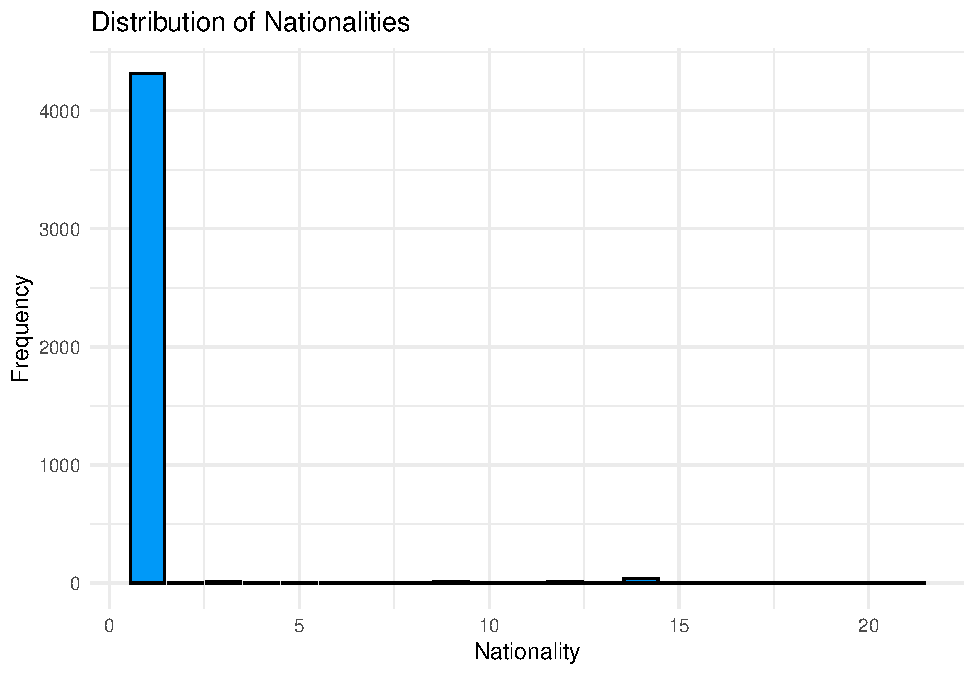
\includegraphics{midterm_files/figure-latex/unnamed-chunk-6-1.pdf}

\begin{Shaded}
\begin{Highlighting}[]
\CommentTok{\#Course}
\NormalTok{knitr}\SpecialCharTok{::}\FunctionTok{kable}\NormalTok{(}\FunctionTok{count}\NormalTok{(df, }\StringTok{\textquotesingle{}Program\textquotesingle{}}\NormalTok{), }\AttributeTok{col.names =} \FunctionTok{c}\NormalTok{(}\StringTok{"Program Number"}\NormalTok{, }\StringTok{"Frequency"}\NormalTok{), }\AttributeTok{align =} \StringTok{"c"}\NormalTok{) }\SpecialCharTok{\%\textgreater{}\%}
  \FunctionTok{kable\_material}\NormalTok{(}\FunctionTok{c}\NormalTok{(}\StringTok{"striped"}\NormalTok{, }\StringTok{"hover"}\NormalTok{)) }\SpecialCharTok{\%\textgreater{}\%} 
 \FunctionTok{scroll\_box}\NormalTok{(}\AttributeTok{width =} \StringTok{"500px"}\NormalTok{, }\AttributeTok{height =} \StringTok{"1000px"}\NormalTok{)}
\end{Highlighting}
\end{Shaded}

\begin{table}
\centering
\begin{tabular}{c|c}
\hline
Program Number & Frequency\\
\hline
1 & 12\\
\hline
2 & 215\\
\hline
3 & 215\\
\hline
4 & 210\\
\hline
5 & 226\\
\hline
6 & 337\\
\hline
7 & 170\\
\hline
8 & 141\\
\hline
9 & 380\\
\hline
10 & 355\\
\hline
11 & 252\\
\hline
12 & 766\\
\hline
13 & 86\\
\hline
14 & 268\\
\hline
15 & 331\\
\hline
16 & 192\\
\hline
17 & 268\\
\hline
\end{tabular}
\end{table}

\begin{Shaded}
\begin{Highlighting}[]
\FunctionTok{ggplot}\NormalTok{(df, }\FunctionTok{aes}\NormalTok{(Program)) }\SpecialCharTok{+}
  \FunctionTok{geom\_bar}\NormalTok{(}\AttributeTok{color =} \StringTok{"\#000000"}\NormalTok{, }\AttributeTok{fill =} \StringTok{"\#0099F8"}\NormalTok{) }\SpecialCharTok{+} \FunctionTok{theme\_minimal}\NormalTok{()}\SpecialCharTok{+}
  \FunctionTok{labs}\NormalTok{(}\AttributeTok{y=}\StringTok{"Frequency"}\NormalTok{, }\AttributeTok{title=}\StringTok{"Distribution of Programs"}\NormalTok{)}
\end{Highlighting}
\end{Shaded}

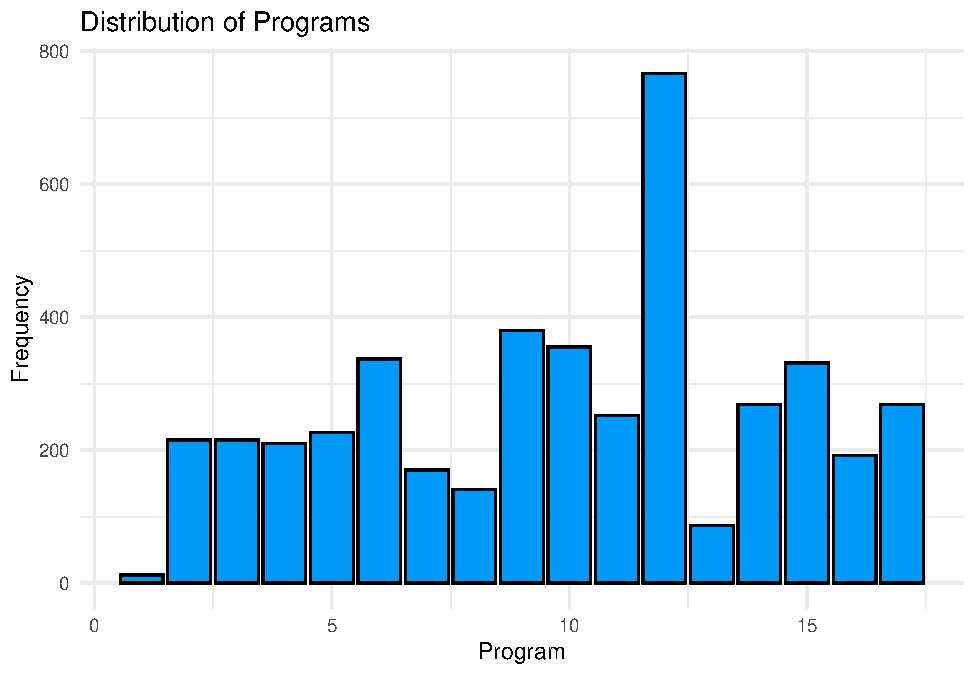
\includegraphics{midterm_files/figure-latex/unnamed-chunk-7-1.pdf}

\begin{Shaded}
\begin{Highlighting}[]
\CommentTok{\#Previous qualification}
\NormalTok{knitr}\SpecialCharTok{::}\FunctionTok{kable}\NormalTok{(}\FunctionTok{count}\NormalTok{(df, }\StringTok{\textquotesingle{}Prev\_quali\textquotesingle{}}\NormalTok{), }\AttributeTok{col.names =} \FunctionTok{c}\NormalTok{(}\StringTok{"Previous Qualification Number"}\NormalTok{, }\StringTok{"Frequency"}\NormalTok{), }\AttributeTok{align =} \StringTok{"c"}\NormalTok{) }\SpecialCharTok{\%\textgreater{}\%}
  \FunctionTok{kable\_material}\NormalTok{(}\FunctionTok{c}\NormalTok{(}\StringTok{"striped"}\NormalTok{, }\StringTok{"hover"}\NormalTok{)) }\SpecialCharTok{\%\textgreater{}\%} 
 \FunctionTok{scroll\_box}\NormalTok{(}\AttributeTok{width =} \StringTok{"500px"}\NormalTok{, }\AttributeTok{height =} \StringTok{"1000px"}\NormalTok{)}
\end{Highlighting}
\end{Shaded}

\begin{table}
\centering
\begin{tabular}{c|c}
\hline
Previous Qualification Number & Frequency\\
\hline
1 & 3717\\
\hline
2 & 23\\
\hline
3 & 126\\
\hline
4 & 8\\
\hline
5 & 1\\
\hline
6 & 16\\
\hline
7 & 11\\
\hline
8 & 4\\
\hline
9 & 45\\
\hline
10 & 1\\
\hline
11 & 2\\
\hline
12 & 162\\
\hline
13 & 7\\
\hline
14 & 219\\
\hline
15 & 40\\
\hline
16 & 36\\
\hline
17 & 6\\
\hline
\end{tabular}
\end{table}

\begin{Shaded}
\begin{Highlighting}[]
\FunctionTok{ggplot}\NormalTok{(df, }\FunctionTok{aes}\NormalTok{(Prev\_quali)) }\SpecialCharTok{+}
  \FunctionTok{geom\_bar}\NormalTok{(}\AttributeTok{color =} \StringTok{"\#000000"}\NormalTok{, }\AttributeTok{fill =} \StringTok{"\#0099F8"}\NormalTok{) }\SpecialCharTok{+} \FunctionTok{theme\_minimal}\NormalTok{()}\SpecialCharTok{+}
  \FunctionTok{labs}\NormalTok{(}\AttributeTok{x =} \StringTok{"Previous Qualification"}\NormalTok{, }\AttributeTok{y=}\StringTok{"Frequency"}\NormalTok{, }\AttributeTok{title=}\StringTok{"Distribution of Previous Qualifications"}\NormalTok{)}
\end{Highlighting}
\end{Shaded}

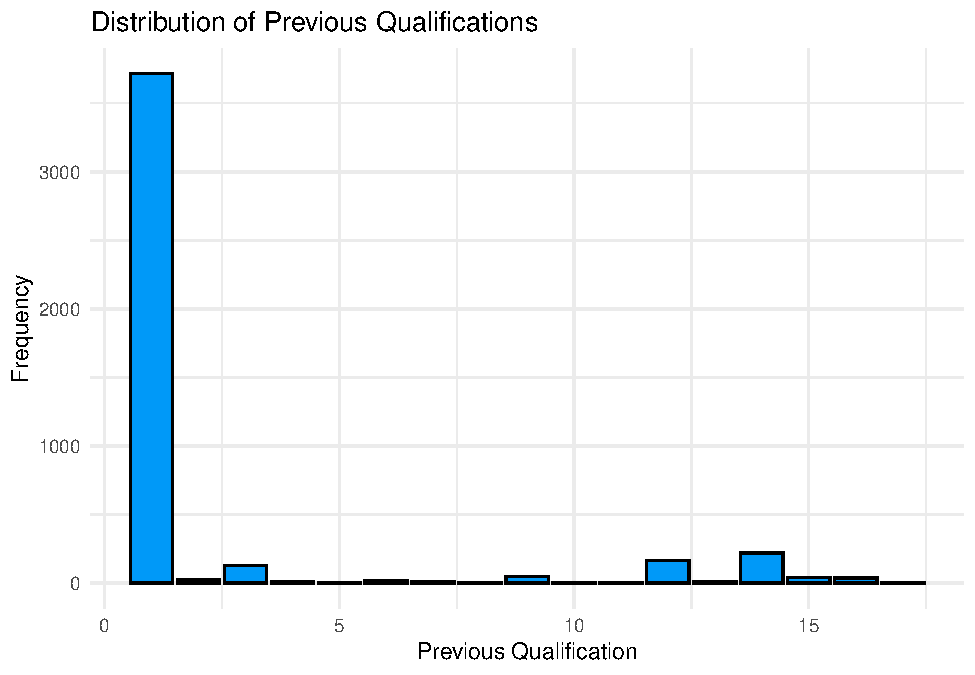
\includegraphics{midterm_files/figure-latex/unnamed-chunk-8-1.pdf}

\begin{Shaded}
\begin{Highlighting}[]
\CommentTok{\#Mother\textquotesingle{}s qualification}
\NormalTok{knitr}\SpecialCharTok{::}\FunctionTok{kable}\NormalTok{(}\FunctionTok{count}\NormalTok{(df, }\StringTok{\textquotesingle{}Mom\_quali\textquotesingle{}}\NormalTok{), }\AttributeTok{col.names =} \FunctionTok{c}\NormalTok{(}\StringTok{"Mother\textquotesingle{}s Qualification Number"}\NormalTok{, }\StringTok{"Frequency"}\NormalTok{), }\AttributeTok{align =} \StringTok{"c"}\NormalTok{) }\SpecialCharTok{\%\textgreater{}\%}
  \FunctionTok{kable\_material}\NormalTok{(}\FunctionTok{c}\NormalTok{(}\StringTok{"striped"}\NormalTok{, }\StringTok{"hover"}\NormalTok{)) }\SpecialCharTok{\%\textgreater{}\%} 
 \FunctionTok{scroll\_box}\NormalTok{(}\AttributeTok{width =} \StringTok{"500px"}\NormalTok{, }\AttributeTok{height =} \StringTok{"1000px"}\NormalTok{)}
\end{Highlighting}
\end{Shaded}

\begin{table}
\centering
\begin{tabular}{c|c}
\hline
Mother's Qualification Number & Frequency\\
\hline
1 & 1069\\
\hline
2 & 83\\
\hline
3 & 438\\
\hline
4 & 49\\
\hline
5 & 21\\
\hline
6 & 4\\
\hline
7 & 8\\
\hline
8 & 3\\
\hline
9 & 3\\
\hline
10 & 42\\
\hline
11 & 2\\
\hline
12 & 1\\
\hline
13 & 953\\
\hline
14 & 1\\
\hline
15 & 1\\
\hline
16 & 1\\
\hline
17 & 3\\
\hline
18 & 3\\
\hline
19 & 130\\
\hline
20 & 3\\
\hline
21 & 3\\
\hline
22 & 1009\\
\hline
23 & 562\\
\hline
24 & 8\\
\hline
25 & 9\\
\hline
26 & 6\\
\hline
27 & 4\\
\hline
28 & 4\\
\hline
29 & 1\\
\hline
\end{tabular}
\end{table}

\begin{Shaded}
\begin{Highlighting}[]
\FunctionTok{ggplot}\NormalTok{(df, }\FunctionTok{aes}\NormalTok{(Mom\_quali)) }\SpecialCharTok{+}
  \FunctionTok{geom\_bar}\NormalTok{(}\AttributeTok{color =} \StringTok{"\#000000"}\NormalTok{, }\AttributeTok{fill =} \StringTok{"\#0099F8"}\NormalTok{) }\SpecialCharTok{+} \FunctionTok{theme\_minimal}\NormalTok{()}\SpecialCharTok{+}
  \FunctionTok{labs}\NormalTok{(}\AttributeTok{x =} \StringTok{"Mother\textquotesingle{}s Qualification"}\NormalTok{, }\AttributeTok{y=}\StringTok{"Frequency"}\NormalTok{, }\AttributeTok{title=}\StringTok{"Distribution of Mother\textquotesingle{}s Qualifications"}\NormalTok{)}
\end{Highlighting}
\end{Shaded}

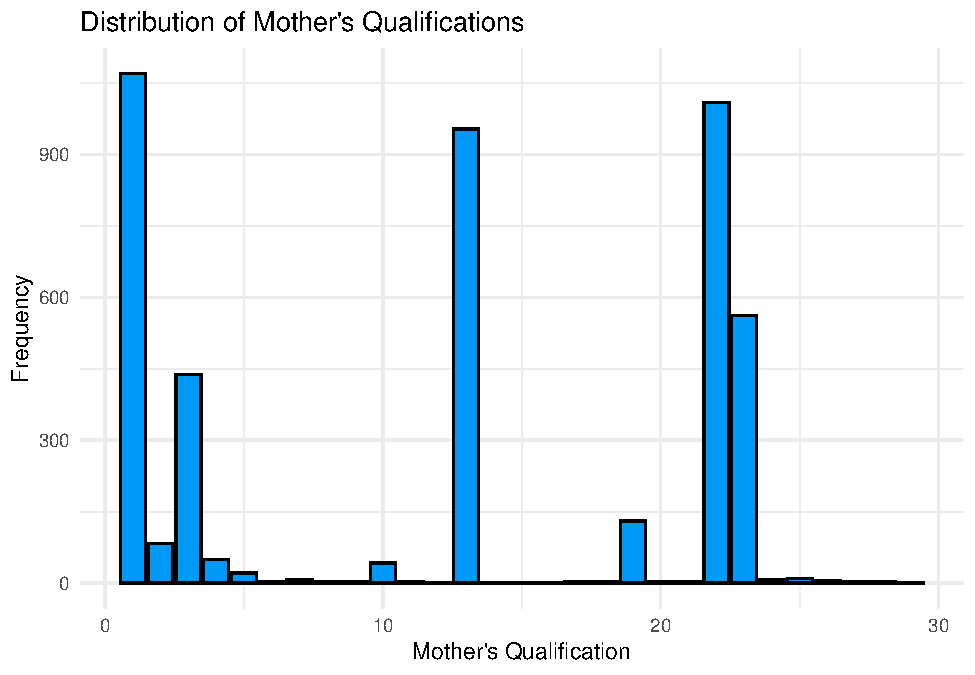
\includegraphics{midterm_files/figure-latex/unnamed-chunk-9-1.pdf}

\begin{Shaded}
\begin{Highlighting}[]
\CommentTok{\#Father\textquotesingle{}s qualification}
\NormalTok{knitr}\SpecialCharTok{::}\FunctionTok{kable}\NormalTok{(}\FunctionTok{count}\NormalTok{(df, }\StringTok{\textquotesingle{}Dad\_quali\textquotesingle{}}\NormalTok{), }\AttributeTok{col.names =} \FunctionTok{c}\NormalTok{(}\StringTok{"Father\textquotesingle{}s Qualification Number"}\NormalTok{, }\StringTok{"Frequency"}\NormalTok{), }\AttributeTok{align =} \StringTok{"c"}\NormalTok{) }\SpecialCharTok{\%\textgreater{}\%}
  \FunctionTok{kable\_material}\NormalTok{(}\FunctionTok{c}\NormalTok{(}\StringTok{"striped"}\NormalTok{, }\StringTok{"hover"}\NormalTok{)) }\SpecialCharTok{\%\textgreater{}\%} 
 \FunctionTok{scroll\_box}\NormalTok{(}\AttributeTok{width =} \StringTok{"500px"}\NormalTok{, }\AttributeTok{height =} \StringTok{"1000px"}\NormalTok{)}
\end{Highlighting}
\end{Shaded}

\begin{table}
\centering
\begin{tabular}{c|c}
\hline
Father's Qualification Number & Frequency\\
\hline
1 & 904\\
\hline
2 & 68\\
\hline
3 & 282\\
\hline
4 & 39\\
\hline
5 & 18\\
\hline
6 & 2\\
\hline
7 & 5\\
\hline
8 & 2\\
\hline
9 & 10\\
\hline
10 & 38\\
\hline
11 & 1\\
\hline
12 & 4\\
\hline
13 & 1\\
\hline
14 & 968\\
\hline
15 & 1\\
\hline
16 & 4\\
\hline
17 & 1\\
\hline
18 & 2\\
\hline
19 & 1\\
\hline
20 & 3\\
\hline
21 & 4\\
\hline
22 & 1\\
\hline
23 & 1\\
\hline
24 & 112\\
\hline
25 & 2\\
\hline
26 & 8\\
\hline
27 & 1209\\
\hline
28 & 702\\
\hline
29 & 20\\
\hline
30 & 5\\
\hline
31 & 2\\
\hline
32 & 1\\
\hline
33 & 2\\
\hline
34 & 1\\
\hline
\end{tabular}
\end{table}

\begin{Shaded}
\begin{Highlighting}[]
\FunctionTok{ggplot}\NormalTok{(df, }\FunctionTok{aes}\NormalTok{(Dad\_quali)) }\SpecialCharTok{+}
  \FunctionTok{geom\_bar}\NormalTok{(}\AttributeTok{color =} \StringTok{"\#000000"}\NormalTok{, }\AttributeTok{fill =} \StringTok{"\#0099F8"}\NormalTok{) }\SpecialCharTok{+} \FunctionTok{theme\_minimal}\NormalTok{()}\SpecialCharTok{+}
  \FunctionTok{labs}\NormalTok{(}\AttributeTok{x =} \StringTok{"Father\textquotesingle{}s Qualification"}\NormalTok{, }\AttributeTok{y=}\StringTok{"Frequency"}\NormalTok{, }\AttributeTok{title=}\StringTok{"Distribution of Father\textquotesingle{}s Qualifications"}\NormalTok{)}
\end{Highlighting}
\end{Shaded}

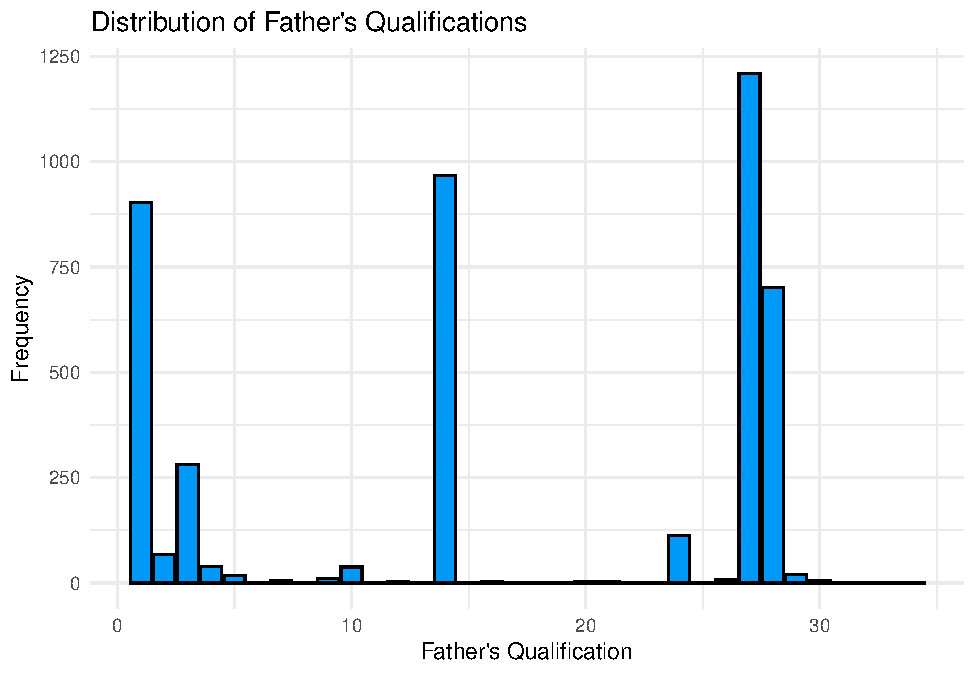
\includegraphics{midterm_files/figure-latex/unnamed-chunk-10-1.pdf}

\begin{Shaded}
\begin{Highlighting}[]
\CommentTok{\#Gender}
\NormalTok{knitr}\SpecialCharTok{::}\FunctionTok{kable}\NormalTok{(}\FunctionTok{count}\NormalTok{(df, }\StringTok{\textquotesingle{}Gender\textquotesingle{}}\NormalTok{), }\AttributeTok{col.names =} \FunctionTok{c}\NormalTok{(}\StringTok{"Gender"}\NormalTok{, }\StringTok{"Frequency"}\NormalTok{), }\AttributeTok{align =} \StringTok{"c"}\NormalTok{) }\SpecialCharTok{\%\textgreater{}\%}
  \FunctionTok{kable\_material}\NormalTok{(}\FunctionTok{c}\NormalTok{(}\StringTok{"striped"}\NormalTok{, }\StringTok{"hover"}\NormalTok{))}
\end{Highlighting}
\end{Shaded}

\begin{table}
\centering
\begin{tabular}{c|c}
\hline
Gender & Frequency\\
\hline
0 & 2868\\
\hline
1 & 1556\\
\hline
\end{tabular}
\end{table}

\begin{Shaded}
\begin{Highlighting}[]
\CommentTok{\#Age}
\NormalTok{knitr}\SpecialCharTok{::}\FunctionTok{kable}\NormalTok{(}\FunctionTok{count}\NormalTok{(df, }\StringTok{\textquotesingle{}Age\textquotesingle{}}\NormalTok{), }\AttributeTok{col.names =} \FunctionTok{c}\NormalTok{(}\StringTok{"Age"}\NormalTok{, }\StringTok{"Frequency"}\NormalTok{), }\AttributeTok{align =} \StringTok{"c"}\NormalTok{) }\SpecialCharTok{\%\textgreater{}\%}
  \FunctionTok{kable\_material}\NormalTok{(}\FunctionTok{c}\NormalTok{(}\StringTok{"striped"}\NormalTok{, }\StringTok{"hover"}\NormalTok{)) }\SpecialCharTok{\%\textgreater{}\%} 
 \FunctionTok{scroll\_box}\NormalTok{(}\AttributeTok{width =} \StringTok{"500px"}\NormalTok{, }\AttributeTok{height =} \StringTok{"1000px"}\NormalTok{)}
\end{Highlighting}
\end{Shaded}

\begin{table}
\centering
\begin{tabular}{c|c}
\hline
Age & Frequency\\
\hline
17 & 5\\
\hline
18 & 1036\\
\hline
19 & 911\\
\hline
20 & 599\\
\hline
21 & 322\\
\hline
22 & 174\\
\hline
23 & 108\\
\hline
24 & 131\\
\hline
25 & 93\\
\hline
26 & 94\\
\hline
27 & 91\\
\hline
28 & 83\\
\hline
29 & 66\\
\hline
30 & 49\\
\hline
31 & 55\\
\hline
32 & 61\\
\hline
33 & 45\\
\hline
34 & 60\\
\hline
35 & 49\\
\hline
36 & 35\\
\hline
37 & 42\\
\hline
38 & 29\\
\hline
39 & 38\\
\hline
40 & 23\\
\hline
41 & 31\\
\hline
42 & 13\\
\hline
43 & 25\\
\hline
44 & 21\\
\hline
45 & 22\\
\hline
46 & 12\\
\hline
47 & 18\\
\hline
48 & 11\\
\hline
49 & 13\\
\hline
50 & 16\\
\hline
51 & 7\\
\hline
52 & 4\\
\hline
53 & 7\\
\hline
54 & 7\\
\hline
55 & 5\\
\hline
57 & 2\\
\hline
58 & 3\\
\hline
59 & 3\\
\hline
60 & 2\\
\hline
61 & 1\\
\hline
62 & 1\\
\hline
70 & 1\\
\hline
\end{tabular}
\end{table}

\begin{Shaded}
\begin{Highlighting}[]
\FunctionTok{ggplot}\NormalTok{(df, }\FunctionTok{aes}\NormalTok{(Age)) }\SpecialCharTok{+}
  \FunctionTok{geom\_histogram}\NormalTok{(}\AttributeTok{bins =} \DecValTok{34}\NormalTok{, }\AttributeTok{color =} \StringTok{"\#000000"}\NormalTok{, }\AttributeTok{fill =} \StringTok{"\#0099F8"}\NormalTok{) }\SpecialCharTok{+} \FunctionTok{theme\_minimal}\NormalTok{()}\SpecialCharTok{+}
  \FunctionTok{labs}\NormalTok{(}\AttributeTok{y=}\StringTok{"Frequency"}\NormalTok{, }\AttributeTok{title=}\StringTok{"Distribution of Age"}\NormalTok{)}
\end{Highlighting}
\end{Shaded}

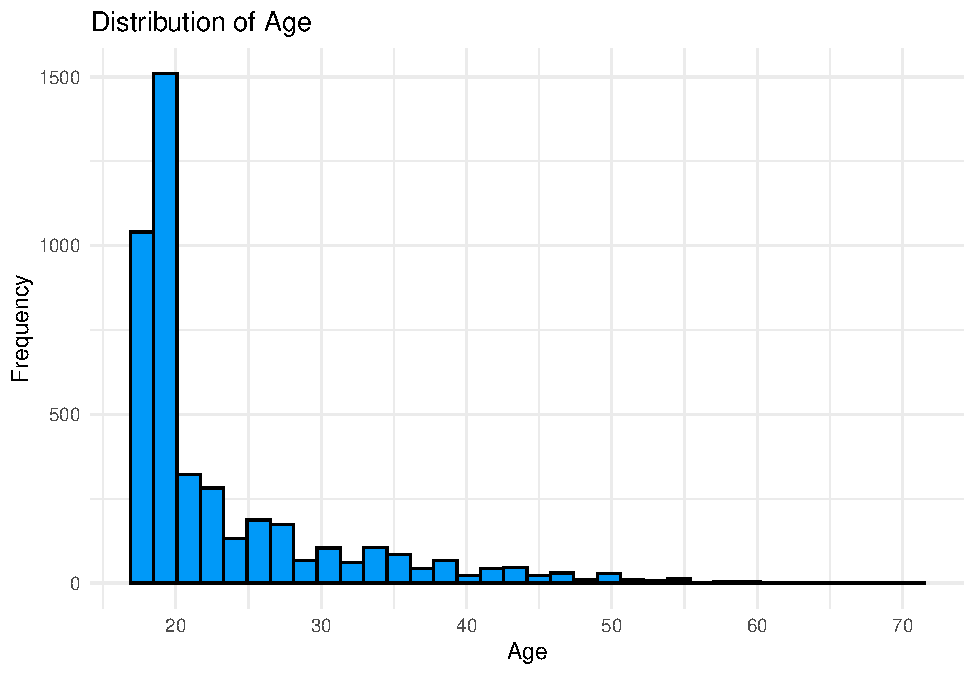
\includegraphics{midterm_files/figure-latex/unnamed-chunk-12-1.pdf}

\begin{Shaded}
\begin{Highlighting}[]
\CommentTok{\#Unemployment Rates}
\NormalTok{knitr}\SpecialCharTok{::}\FunctionTok{kable}\NormalTok{(}\FunctionTok{count}\NormalTok{(df, }\StringTok{\textquotesingle{}Unemp\_rate\textquotesingle{}}\NormalTok{), }\AttributeTok{col.names =} \FunctionTok{c}\NormalTok{(}\StringTok{"Unemployment Rate"}\NormalTok{, }\StringTok{"Frequency"}\NormalTok{), }\AttributeTok{align =} \StringTok{"c"}\NormalTok{) }\SpecialCharTok{\%\textgreater{}\%}
  \FunctionTok{kable\_material}\NormalTok{(}\FunctionTok{c}\NormalTok{(}\StringTok{"striped"}\NormalTok{, }\StringTok{"hover"}\NormalTok{)) }\SpecialCharTok{\%\textgreater{}\%} 
 \FunctionTok{scroll\_box}\NormalTok{(}\AttributeTok{width =} \StringTok{"500px"}\NormalTok{, }\AttributeTok{height =} \StringTok{"1000px"}\NormalTok{)}
\end{Highlighting}
\end{Shaded}

\begin{table}
\centering
\begin{tabular}{c|c}
\hline
Unemployment Rate & Frequency\\
\hline
7.6 & 571\\
\hline
8.9 & 368\\
\hline
9.4 & 533\\
\hline
10.8 & 525\\
\hline
11.1 & 414\\
\hline
12.4 & 445\\
\hline
12.7 & 419\\
\hline
13.9 & 390\\
\hline
15.5 & 397\\
\hline
16.2 & 362\\
\hline
\end{tabular}
\end{table}

\begin{Shaded}
\begin{Highlighting}[]
\FunctionTok{ggplot}\NormalTok{(df, }\FunctionTok{aes}\NormalTok{(Unemp\_rate)) }\SpecialCharTok{+}
  \FunctionTok{geom\_histogram}\NormalTok{(}\AttributeTok{bins =} \DecValTok{15}\NormalTok{, }\AttributeTok{color =} \StringTok{"\#000000"}\NormalTok{, }\AttributeTok{fill =} \StringTok{"\#0099F8"}\NormalTok{) }\SpecialCharTok{+} \FunctionTok{theme\_minimal}\NormalTok{()}\SpecialCharTok{+}
  \FunctionTok{labs}\NormalTok{(}\AttributeTok{x =} \StringTok{"Unemployment Rate"}\NormalTok{, }\AttributeTok{y=}\StringTok{"Frequency"}\NormalTok{, }\AttributeTok{title=}\StringTok{"Distribution of Unemployment Rates"}\NormalTok{)}
\end{Highlighting}
\end{Shaded}

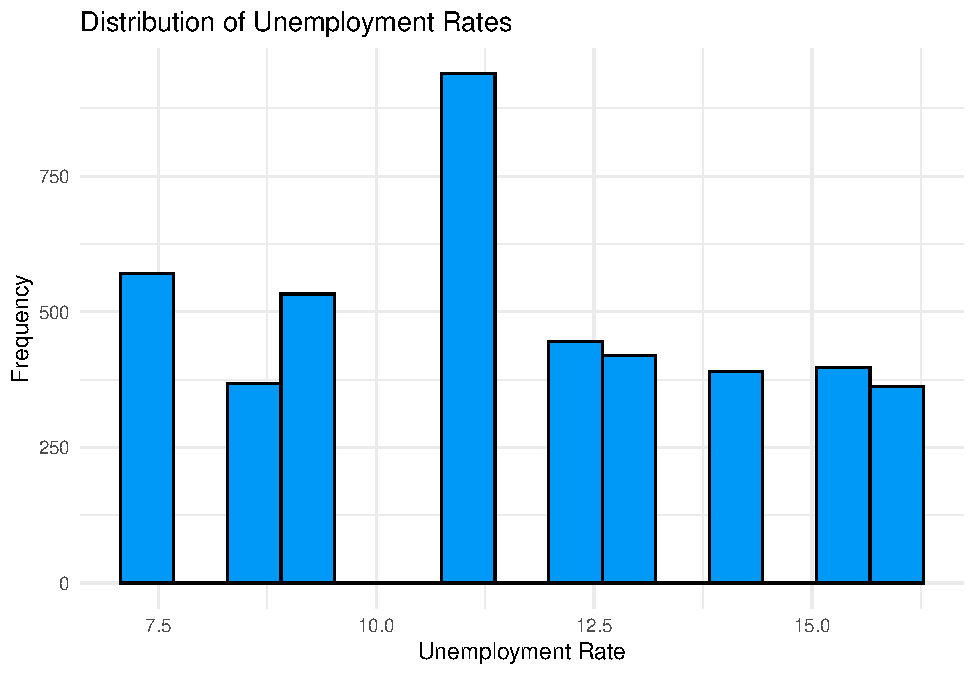
\includegraphics{midterm_files/figure-latex/unnamed-chunk-13-1.pdf}

\begin{Shaded}
\begin{Highlighting}[]
\CommentTok{\#Life Expectancy (in years)}
\NormalTok{knitr}\SpecialCharTok{::}\FunctionTok{kable}\NormalTok{(}\FunctionTok{count}\NormalTok{(df, }\StringTok{\textquotesingle{}Life\_expectancy\textquotesingle{}}\NormalTok{), }\AttributeTok{col.names =} \FunctionTok{c}\NormalTok{(}\StringTok{"Life Expectancy"}\NormalTok{, }\StringTok{"Frequency"}\NormalTok{), }\AttributeTok{align =} \StringTok{"c"}\NormalTok{) }\SpecialCharTok{\%\textgreater{}\%}
  \FunctionTok{kable\_material}\NormalTok{(}\FunctionTok{c}\NormalTok{(}\StringTok{"striped"}\NormalTok{, }\StringTok{"hover"}\NormalTok{)) }\SpecialCharTok{\%\textgreater{}\%} 
 \FunctionTok{scroll\_box}\NormalTok{(}\AttributeTok{width =} \StringTok{"500px"}\NormalTok{, }\AttributeTok{height =} \StringTok{"1000px"}\NormalTok{)}
\end{Highlighting}
\end{Shaded}

\begin{table}
\centering
\begin{tabular}{c|c}
\hline
Life Expectancy & Frequency\\
\hline
59.72000 & 5\\
\hline
61.16600 & 2\\
\hline
62.44800 & 2\\
\hline
68.52300 & 14\\
\hline
70.93500 & 3\\
\hline
71.82732 & 3\\
\hline
73.08390 & 2\\
\hline
74.20200 & 2\\
\hline
75.33800 & 38\\
\hline
75.60732 & 2\\
\hline
76.00400 & 13\\
\hline
76.28293 & 1\\
\hline
76.75200 & 1\\
\hline
77.61100 & 1\\
\hline
77.83200 & 1\\
\hline
81.20488 & 1\\
\hline
81.29268 & 2\\
\hline
81.67561 & 4314\\
\hline
82.11220 & 1\\
\hline
83.49756 & 3\\
\hline
83.83171 & 13\\
\hline
\end{tabular}
\end{table}

\begin{Shaded}
\begin{Highlighting}[]
\FunctionTok{ggplot}\NormalTok{(df, }\FunctionTok{aes}\NormalTok{(Life\_expectancy)) }\SpecialCharTok{+}
  \FunctionTok{geom\_histogram}\NormalTok{(}\AttributeTok{bins =} \DecValTok{15}\NormalTok{, }\AttributeTok{color =} \StringTok{"\#000000"}\NormalTok{, }\AttributeTok{fill =} \StringTok{"\#0099F8"}\NormalTok{) }\SpecialCharTok{+} \FunctionTok{theme\_minimal}\NormalTok{()}\SpecialCharTok{+}
  \FunctionTok{labs}\NormalTok{(}\AttributeTok{x =} \StringTok{"Life Expectancy"}\NormalTok{, }\AttributeTok{y=}\StringTok{"Frequency"}\NormalTok{, }\AttributeTok{title=}\StringTok{"Distribution of Life Expectancy (in years)"}\NormalTok{)}
\end{Highlighting}
\end{Shaded}

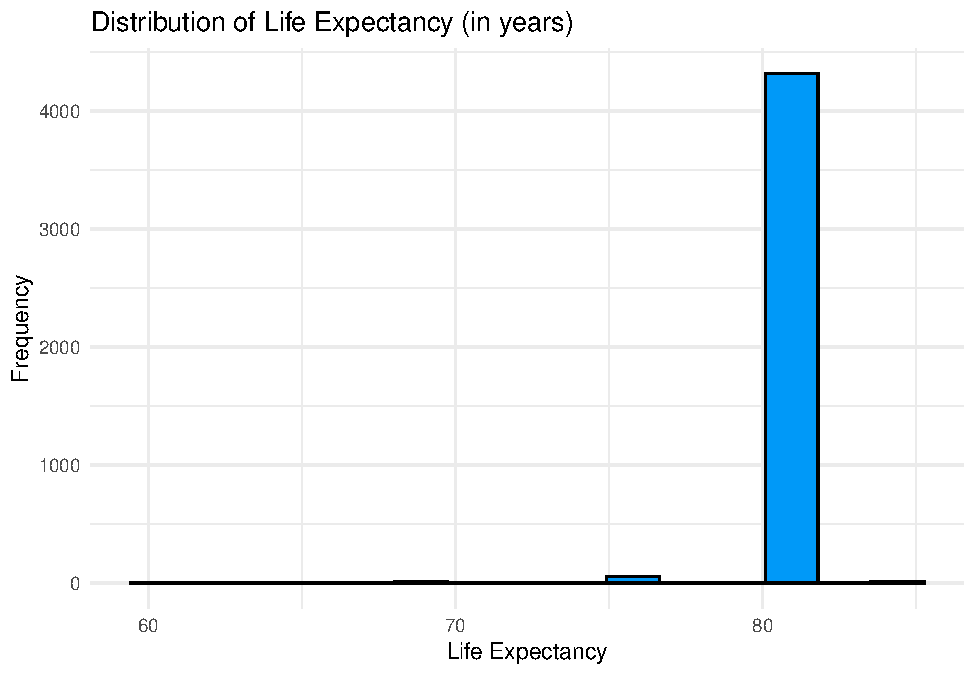
\includegraphics{midterm_files/figure-latex/unnamed-chunk-14-1.pdf}

\begin{Shaded}
\begin{Highlighting}[]
\CommentTok{\# Target}
\NormalTok{target\_df }\OtherTok{\textless{}{-}} \FunctionTok{count}\NormalTok{(df, }\StringTok{\textquotesingle{}Target\textquotesingle{}}\NormalTok{)}
\FunctionTok{ggplot}\NormalTok{(target\_df, }\FunctionTok{aes}\NormalTok{(}\AttributeTok{x=}\StringTok{""}\NormalTok{, }\AttributeTok{y=}\NormalTok{freq, }\AttributeTok{fill=}\NormalTok{Target)) }\SpecialCharTok{+}
  \FunctionTok{geom\_bar}\NormalTok{(}\AttributeTok{stat=}\StringTok{"identity"}\NormalTok{, }\AttributeTok{width=}\DecValTok{1}\NormalTok{, }\AttributeTok{color=}\StringTok{"white"}\NormalTok{) }\SpecialCharTok{+}
  \FunctionTok{coord\_polar}\NormalTok{(}\StringTok{"y"}\NormalTok{, }\AttributeTok{start=}\DecValTok{0}\NormalTok{) }\SpecialCharTok{+}
  \FunctionTok{theme\_void}\NormalTok{() }\SpecialCharTok{+} 
  \FunctionTok{scale\_fill\_brewer}\NormalTok{(}\AttributeTok{palette=}\StringTok{"Blues"}\NormalTok{) }\SpecialCharTok{+} 
  \FunctionTok{labs}\NormalTok{(}\AttributeTok{title =} \StringTok{"Distribution of students who have graduated vs dropped out vs enrolled"}\NormalTok{)}
\end{Highlighting}
\end{Shaded}

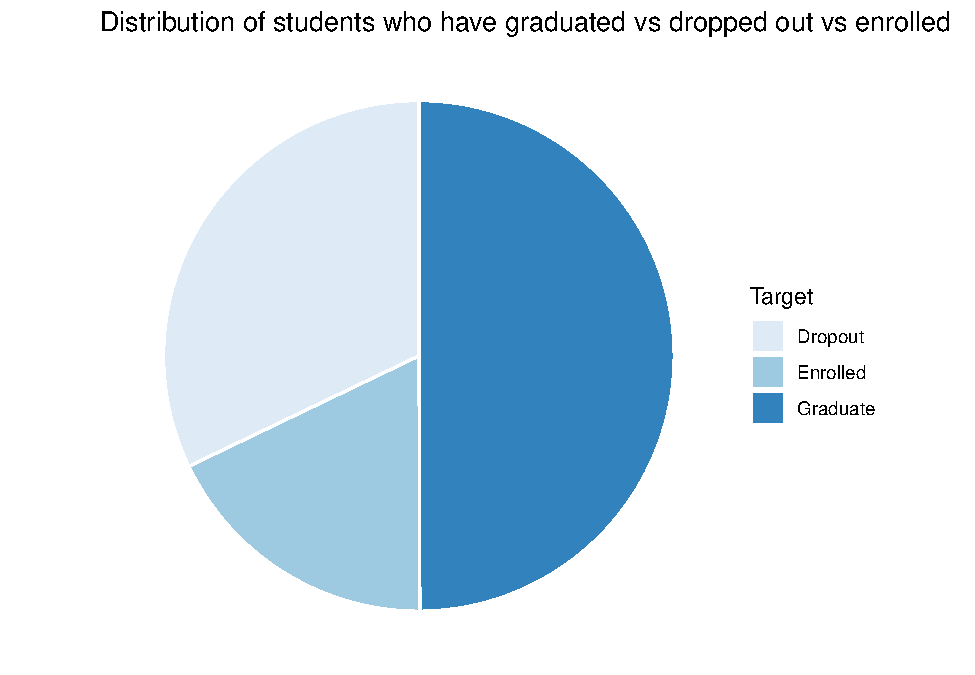
\includegraphics{midterm_files/figure-latex/unnamed-chunk-15-1.pdf}

\end{document}
